%\documentclass[a4paper, twoside]{article}
\setcounter{secnumdepth}{5}
\setcounter{tocdepth}{5}
\usepackage[english]{babel}
\usepackage{textcomp}
\usepackage{amsmath,amsthm,amsfonts,amssymb,epsfig}
\usepackage{array}
\usepackage{datetime}
\usepackage{lipsum}% http://ctan.org/pkg/lipsum
\usepackage[left=1.1in,top=1in,right=1.1in]{geometry}% http://ctan.org/pkg/geometry
\usepackage{listings}% http://ctan.org/pkg/listings
\usepackage{spverbatim}
\usepackage{hyperref}
\usepackage{microtype}
\hypersetup{colorlinks=true, urlcolor=black, linkcolor=black}
\usepackage{graphicx}
\graphicspath{ {images/} }
\usepackage{parskip}
\usepackage{titlesec} %used for diminishing heading sizes
\usepackage[square, sort, comma, numbers]{natbib} %%uses titles for cited references
\usepackage[fit]{truncate}
\usepackage{fancyhdr}
\pagestyle{fancy}
\fancyhead{}
\fancyhead[RO, RE]{\thepage}
\fancyhead[LO, LE]{\rightmark}
\renewcommand{\sectionmark}[1]{\markboth{}{\textsc{\thesection~#1}}}
\fancyfoot[C]{}%hide footer
\usepackage{xcolor} 
\usepackage[scaled=1]{couriers}

\xdefinecolor{gray}{rgb}{0.6,0.6,0.6} 
\documentclass[twoside]{article}
\usepackage[top=1in, left=0.5in, right=0.5in, bottom=0.5in,paperheight=8.5in,paperwidth=5.5in]{geometry}
\setcounter{secnumdepth}{5}
\setcounter{tocdepth}{5}
\usepackage[english]{babel}
\usepackage{textcomp}
\usepackage{amsmath,amsthm,amsfonts,amssymb,epsfig}
\usepackage{array}
\usepackage{datetime}
\usepackage{lipsum}% http://ctan.org/pkg/lipsum
\usepackage{listings}% http://ctan.org/pkg/listings
\usepackage{spverbatim}
\usepackage[hidelinks]{hyperref}
\Urlmuskip=0mu plus 1mu\relax %needed to make long URLs break nicely
\usepackage{microtype}
\hypersetup{colorlinks=false}
\usepackage{graphicx}
\graphicspath{ {images/} }
\usepackage{parskip}
\usepackage{titlesec} %used for diminishing heading sizes
\titleformat{\section}{\normalfont\bfseries}{\thesection}{1em}{}
\titlespacing*{\section}{0pt}{*2}{0pt}
\titlespacing*{\subsection}{0pt}{*2}{0pt}
\usepackage[square, sort, comma, numbers]{natbib} %%uses titles for cited references
\usepackage[fit]{truncate}
\usepackage{fancyhdr}
\pagestyle{fancy}
\renewcommand{\sectionmark}[1]{\markboth{#1}{}}
\fancyhead{}
\fancyhead[OR]{\leftmark \hspace{0.1cm}  $\vert$ \hspace{0.1cm}  \thepage}
\fancyhead[EL]{\thepage \hspace{0.1cm} $\vert$ \hspace{0.1cm} \leftmark}
\fancyfoot[C]{}%hide footer
\usepackage{xcolor} 
\usepackage[scaled=1]{couriers}
\usepackage{graphicx}
\xdefinecolor{gray}{rgb}{0.6,0.6,0.6} 
\usepackage{setspace}
\usepackage{adjustbox} 

  %settings for printed booklets - comment out by default, uncomment for print and comment out line above. don't save this change! "conf_top" should be default

\defcitealias{lenet}{Gradient-Based Learning Applied to Document Recognition}

\defcitealias{alexnet}{ImageNet Classification with Deep Convolutional Neural Networks}

\defcitealias{vgg}{Very Deep Convolutional Networks for Large-Scale Image Recognition}

\defcitealias{googlenet}{Going Deeper with Convolutions}

\defcitealias{inceptionbn}{Batch Normalization: Accelerating Deep Network Training by Reducing Internal Covariate Shift}

\defcitealias{resnet}{Deep Residual Learning for Image Recognition}

\defcitealias{bergstra-bengio}{Random Search for Hyper-parameter Optimization}

\defcitealias{mnist}{The MNIST Database}

\defcitealias{h2o_DL_booklet}{Deep Learning with H2O Booklet}


\usepackage{float}
\usepackage{bibentry}
\usepackage{url}
\def\UrlBreaks{\do\/\do-}


\titleformat*{\section}{\LARGE\bfseries\sffamily}
\titleformat*{\subsection}{\Large\bfseries\sffamily}
\titleformat*{\subsubsection}{\large\bfseries\sffamily}
\titleformat*{\paragraph}{\large\bfseries\sffamily}
\titleformat*{\subparagraph}{\large\bfseries\sffamily}
\renewcommand{\familydefault}{\sfdefault} %sans-serif font



\begin{document}

%----------------------------------------------------------------------
% Definition for "lstlisting" blocks
%----------------------------------------------------------------------
% --- USAGE ---
%
% \begin{lstlisting}[style=R}
% ...
% \end{lstlisting}
%
% % \begin{lstlisting}[style=output}
% ...
% \end{lstlisting}
%----------------------------------------------------------------------

% By default, make listings all black so it's easy to spot the ones that aren't set to a style.
% This is just a debugging technique.
\lstset{backgroundcolor=\color{black}}

% Define scala language first
% ``define'' Scala
\lstdefinelanguage{scala}{
  morekeywords={abstract,case,catch,class,def,%
    do,else,extends,false,final,finally,%
    for,if,implicit,import,match,mixin,%
    new,null,object,override,package,%
    private,protected,requires,return,sealed,%
    super,this,throw,trait,true,try,%
    type,val,var,while,with,yield},
  otherkeywords={=>,<-,<\%,<:,>:,\#,@},
  sensitive=true,
  morecomment=[l]{//},
  morecomment=[n]{/*}{*/},
  morestring=[b]``,
  morestring=[b]',
  morestring=[b]''``
}

\lstdefinestyle{R}{
  language=R,
  frame=single,
  breaklines,
  basicstyle=\ttfamily,
  commentstyle=\textbf,% comment style
  keywordstyle=\ttfamily,
  numbers=left,% display line numbers on the left side 
  numberstyle=\scriptsize,% use small line numbers 
  numbersep=10pt,% space between line numbers and code
  backgroundcolor=\color{white}, 
  showstringspaces=false % don't show spaces as weird char.
}

\lstdefinestyle{python}{
  language=python,
  frame=single,
  breaklines,
  basicstyle=\ttfamily,
  commentstyle=\textsl,% comment style
  keywordstyle=\ttfamily,
  numbers=left,% display line numbers on the left side 
  numberstyle=\scriptsize,% use small line numbers 
  numbersep=10pt,% space between line numbers and code
  backgroundcolor=\color{white}, 
  showstringspaces=false %don't show spaces as weird char.
}

\lstdefinestyle{Scala}{
  language=scala,
  frame=single,
  breaklines,
  basicstyle=\ttfamily,
  commentstyle=\textsl,% comment style
  keywordstyle=\ttfamily,
  numbers=left,% display line numbers on the left side 
  numberstyle=\scriptsize,% use small line numbers 
  numbersep=10pt,% space between line numbers and code
  backgroundcolor=\color{white}, 
  showstringspaces=false % don't show spaces as weird char.
}

\lstdefinestyle{Bash}{
  language=bash,
  frame=single,
  breaklines,
  basicstyle=\ttfamily,
  commentstyle=\textsl,% comment style
  keywordstyle=\ttfamily,
  numbers=left,% display line numbers on the left side 
  numberstyle=\scriptsize,% use small line numbers 
  numbersep=10pt,% space between line numbers and code
  backgroundcolor=\color{white}, 
  showstringspaces=false % don't show spaces as weird char.
}


\definecolor{mygray}{rgb}{0.92,0.92,0.92}

\lstdefinestyle{output}{
  frame=single,
  breaklines,
  basicstyle=\ttfamily,
  numbers=left,% display line numbers on the left side 
  numberstyle=\scriptsize,% use small line numbers 
  numbersep=10pt,% space between line numbers and code
  backgroundcolor=\color{mygray}, 
  showstringspaces=false %don't show spaces as weird char.
}

\newcommand{\waterExampleInR} {
\textbf{Example in R} \\
}

\newcommand{\waterExampleInPython} {
\textbf{Example in Python} \\
}
 %see note for `conf_top_print.tex` above
%% TO DO: Find better templates for R and Python



%----------------------------------------------------------------------
% Definition for "lstlisting" blocks
%----------------------------------------------------------------------
% --- USAGE ---
%
% \begin{lstlisting}[style=R}
% ...
% \end{lstlisting}
%
% % \begin{lstlisting}[style=output}
% ...
% \end{lstlisting}
%----------------------------------------------------------------------

% By default, make listings all black so it's easy to spot the ones that aren't set to a style.
% This is just a debugging technique.
%\lstset{backgroundcolor=\color{black}}

% http://latexcolor.com/
\definecolor{deepblue}{rgb}{0,0,0.5}
\definecolor{deepred}{rgb}{0.6,0,0}
\definecolor{deepgreen}{rgb}{0,0.5,0}
%\definecolor{tan}{rgb}{0.98, 0.92, 0.84}  %antiquewhite
%\definecolor{r_bkgd}{rgb}{1.0, 0.92, 0.8}  %blacnedalmond
\definecolor{py_bkgd}{rgb}{0.94, 0.97, 1.0}  %aliceblue
\definecolor{ashgrey}{rgb}{0.7, 0.75, 0.71}
\definecolor{battleshipgrey}{rgb}{0.52, 0.52, 0.51}
%\definecolor{r_bkgd}{rgb}{0.97, 0.91, 0.81}  %champagne
\definecolor{r_bkgd}{rgb}{0.98, 0.92, 0.84}  %moccasin

\definecolor{Code}{rgb}{0,0,0}
\definecolor{Decorators}{rgb}{0.5,0.5,0.5}
\definecolor{Numbers}{rgb}{0.5,0,0}
\definecolor{MatchingBrackets}{rgb}{0.25,0.5,0.5}
\definecolor{Keywords}{rgb}{0,0,1}
\definecolor{self}{rgb}{0,0,0}
\definecolor{Strings}{rgb}{0,0.63,0}
\definecolor{Comments}{rgb}{0,0.63,1}
\definecolor{Backquotes}{rgb}{0,0,0}
\definecolor{Classname}{rgb}{0,0,0}
\definecolor{FunctionName}{rgb}{0,0,0}
\definecolor{Operators}{rgb}{0,0,0}
\definecolor{Background}{rgb}{0.98,0.98,0.98}

% KEYWORDS
% http://tex.stackexchange.com/questions/186092/how-can-i-delete-non-letter-keywords-such-as
\lstdefinestyle{Scala}{
  language={Scala},
  frame=single,
  breaklines,
  basicstyle=\ttfamily,
  commentstyle=\itshape\color{battleshipgrey},% comment style
  %commentstyle=\textsl,% comment style
  %keywordstyle=\ttfamily\color{deepblue},
  %keywordstyle=\color{WildStrawberry},
  numbers=left,% display line numbers on the left side
  numberstyle=\scriptsize,% use small line numbers
  numbersep=10pt,% space between line numbers and code
  backgroundcolor=\color{white},
  showstringspaces=false,
  stringstyle=\color{deepgreen},
  backgroundcolor=\color{py_bkgd},
  % keywords
  morekeywords={abstract,case,catch,class,def,%
    do,else,extends,false,final,finally,%
    for,if,implicit,import,match,mixin,%
    new,null,object,override,package,%
    private,protected,requires,return,sealed,%
    super,this,throw,trait,true,try,%
    type,val,var,while,with,yield},
  otherkeywords={=>,<-,<\%,<:,>:,\#,@},
  sensitive=true,
  morecomment=[l]{//},
  morecomment=[n]{/*}{*/},
  morestring=[b]``,
  morestring=[b]',
  morestring=[b]''``,
  keywordstyle={\color{Keywords}\bfseries},
}

\lstdefinestyle{R}{
  language={R},
  frame=single,
  breaklines,
  basicstyle=\ttfamily,
  %commentstyle=\textsl\color{Comments},% comment style
  commentstyle=\itshape\color{battleshipgrey},% comment style
  keywordstyle=\ttfamily\color{deepblue},
  numbers=left,% display line numbers on the left side 
  numberstyle=\scriptsize,% use small line numbers 
  numbersep=10pt,% space between line numbers and code
  backgroundcolor=\color{r_bkgd},
  showstringspaces=false,
  stringstyle=\color{deepgreen},
  %morekeywords={TRUE, FALSE, for, if},
  keywordstyle={\color{Keywords}\bfseries},
  keywords={TRUE, FALSE},
  deletekeywords={grid, frame, variable, model, vi, predict, file},
  otherkeywords={!,!=,~,$,*,\&,\%/\%,\%*\%,\%\%,<-,<<-},
  %morekeywords={TRUE, FALSE, list, c}
}



\lstdefinestyle{python}{
  language={Python},
  frame=single,
  breaklines,
  basicstyle=\ttfamily,
  commentstyle=\itshape\color{battleshipgrey},% comment style
  %commentstyle=\textsl,% comment style
  %keywordstyle=\ttfamily\color{deepblue},
  %keywordstyle=\color{WildStrawberry},
  numbers=left,% display line numbers on the left side 
  numberstyle=\scriptsize,% use small line numbers 
  numbersep=10pt,% space between line numbers and code
  backgroundcolor=\color{white},
  showstringspaces=false,
  stringstyle=\color{deepgreen},
  backgroundcolor=\color{py_bkgd},
  % keywords
morekeywords={import,from,class,def,for,while,if,is,in,elif,else,not,and,or,print,break,continue,return,True,False,None,access,as,,del,except,exec,finally,global,import,lambda,pass,print,raise,try,assert},
 keywordstyle={\color{Keywords}\bfseries},
}

\lstdefinestyle{Bash}{
  language=bash,
  frame=single,
  breaklines,
  basicstyle=\ttfamily,
  commentstyle=\textsl,% comment style
  keywordstyle=\ttfamily,
  numbers=left,% display line numbers on the left side
  numberstyle=\scriptsize,% use small line numbers
  numbersep=10pt,% space between line numbers and code
  backgroundcolor=\color{white},
  showstringspaces=false % don't show spaces as weird char.
}

\definecolor{mygray}{rgb}{0.92,0.92,0.92}

\lstdefinestyle{output}{
  frame=single,
  breaklines,
  basicstyle=\ttfamily,
  numbers=left,% display line numbers on the left side 
  numberstyle=\scriptsize,% use small line numbers 
  numbersep=10pt,% space between line numbers and code
  backgroundcolor=\color{mygray},
  showstringspaces=false 
}

\newcommand{\waterExampleInR} {
\textbf{Example in R} \\
}

\newcommand{\waterExampleInPython} {
\textbf{Example in Python} \\
}
  %Use this for online version


\thispagestyle{empty} %removes page number
\newgeometry{bmargin=0cm, hmargin=0cm}


\begin{center}
\textsc{\Large\bf{Deep Learning with Deep Water}}
\bigskip

\line(1,0){250}  %inserts  horizontal line



\bigskip

\textsc{\small{Wen Phan \hspace{4pt} Magnus Stensmo \hspace{4pt} Mateusz Dymczyk  \hspace{4pt} Arno Candel \hspace{4pt} Qiang Kou}}

\textsc{\small{Edited by: Angela Bartz}}

\line(1,0){250}  %inserts  horizontal line

{\url{http://h2o.ai/resources/}}

\normalsize
\bigskip
\monthname \hspace{1pt}  \the\year: First Edition

\bigskip
\end{center}

% commenting out lines image due to print issues, but leaving in for later
%\null\vfill
%\begin{figure}[!b]
%\noindent\makebox[\textwidth]{%
%\centerline{
\includegraphics[width=\paperwidth]{waves.png}}}
%\end{figure}


\newpage
\restoregeometry

\null\vfill %move next text block to lower left of new page

\thispagestyle{empty}%remove pg#
{\raggedright\vfill\ 

Deep Learning with Deep Water\\

by Wen Phan, Magnus Stensmo, \\ 
Mateusz Dymczyk, Arno Candel, \&\ Qiang Kou\\
Edited by: Angela Bartz

\bigskip
Published by H2O.ai, Inc. \\
2307 Leghorn St. \\
Mountain View, CA 94043\\
\bigskip
\textcopyright 2017 H2O.ai, Inc. All Rights Reserved. 
\bigskip

\monthname \hspace{1pt}  \the\year: First Edition
\bigskip

Photos by \textcopyright H2O.ai, Inc. 
\bigskip

All copyrights belong to their respective owners.\\
While every precaution has been taken in the\\
preparation of this book, the publisher and\\
authors assume no responsibility for errors or\\
omissions, or for damages resulting from the\\
use of the information contained herein.\\
\bigskip
Printed in the United States of America. 
}

\newpage
\thispagestyle{empty}%remove pg#

\tableofcontents

%----------------------------------------------------------------------
%----------------------------------------------------------------------

\newpage

\section{Introduction}
This booklet introduces the reader to H2O Deep Water, a framework for GPU-accelerated deep learning on H2O.  H2O Deep Water leverages prominent open source deep learning frameworks, such MXNet, TensorFlow, and Caffe, as backends.  Throughout the booklet, Python examples and code snippets will be provided for the reader.  A quick start is provided to quickly familiarize the reader with the Deep Water Python API and its key features.  A section on image classification is also provided and demonstrates using pre-defined, user-defined, and pre-trained networks.  As part of the H2O platform, Deep Water can take advantage of grid search, model checkpointing, and ensembles, and examples of these are also provided.  This booklet also includes a section describing how Deep Water can be used for unsupervised learning tasks.  Finally, deploying Deep Water models for inference is discussed.  To learn more about the H2O platform, please visit: {\url{docs.h2o.ai}}.

\section{What is H2O?}
\Urlmuskip=0mu plus 1mu\relax %needed to make long URLs break nicely


H2O is fast, scalable, open-source machine learning and deep learning for smarter applications. With H2O, enterprises like PayPal, Nielsen Catalina, Cisco, and others can use all their data without sampling to get accurate predictions faster. Advanced algorithms such as deep learning, boosting, and bagging ensembles are built-in to help application designers create smarter applications through elegant APIs. Some of our initial customers have built powerful domain-specific predictive engines for recommendations, customer churn, propensity to buy, dynamic pricing, and fraud detection for the insurance, healthcare, telecommunications, ad tech, retail, and payment systems industries.

Using in-memory compression, H2O handles billions of data rows in-memory, even with a small cluster. To make it easier for non-engineers to create complete analytic workflows, H2O's platform includes interfaces for R, Python, Scala, Java, JSON, and CoffeeScript/JavaScript, as well as a built-in  web interface, Flow. H2O was built alongside (and on top of) Hadoop and Spark Clusters and typically deploys within minutes.

H2O includes many common machine learning algorithms, such as generalized linear modeling (linear regression, logistic regression, etc.), Na\"{i}ve Bayes, principal components analysis, time series, k-means clustering, and others. H2O also implements best-in-class algorithms at scale, such as distributed random forest, gradient boosting and deep learning. Customers can build thousands of models and compare the results to get the best predictions.

H2O is nurturing a grassroots movement of physicists, mathematicians, and computer scientists to herald the new wave of discovery with data science by collaborating closely with academic researchers and Industrial data scientists. Stanford university giants Stephen Boyd, Trevor Hastie, Rob Tibshirani advise the H2O team on building scalable machine learning algorithms. With hundreds of meetups over the past three years, H2O has become a word-of-mouth phenomenon, growing amongst the data community by a hundred-fold, and is now used by 30,000+ users and is deployed using R, Python, Hadoop, and Spark in 2000+ corporations.

\textbf{Try it out}

\begin{itemize}
\item  Download H2O directly at \mbox{\url{http://h2o.ai/download}}.
\item Install H2O's R package from CRAN at {\url{https://cran.r-project.org/web/packages/h2o/}}. 
\item Install the Python package from PyPI at {\url{https://pypi.python.org/pypi/h2o/}}.

\end{itemize}



\textbf{Join the community}
\begin{itemize}
\item  To learn about our meetups, training sessions, hackathons, and product updates, visit {\url{http://h2o.ai}}. 
\item Visit the open source community forum at {\url{https://groups.google.com/d/forum/h2ostream}}.
\item Join the chat at {\url{https://gitter.im/h2oai/h2o-3}}.
\end{itemize}





\input{generated_buildinfo.tex}

\section{Installation}
At the time of this writing, Deep Water has not yet been officially released.  So the three options for installing and/or using Deep Water are to build from source, to try out the H2O Deep Water Amazon Machine Image (AMI), or to run the H2O Docker Image. 

	\subsection{Build from Source}
		Build instructions can be found here: {\url{https://github.com/h2oai/deepwater}}.  Different build configurations can target different hardware and leverage various linear algebra libraries, including MKL, OpenBLAS, ATLAS, and CUDA.
				
	\subsection{Amazon Machine Image}
		For convenience, H2O.ai releases Deep Water AMIs as a way to try out Deep Water on GPU-enabled Amazon EC2 instances.  We are constantly updating the AMIs.  To get information on the latest AMI and how it use it, please visit the following: {\url{https://github.com/h2oai/deepwater/blob/master/docs/open-tour-dallas/deep-water-ami.md}}.  For more information on AWS GPU instances, please visit the following: {\url{http://docs.aws.amazon.com/AWSEC2/latest/UserGuide/accelerated-computing-instances.html}}.
	
	\subsection{Docker Image}
		H2O has released a GPU-enabled Docker image on Docker Hub. To use this image, you must have a Linux machine with at least one GPU. Docker and nvidia-docker must also be installed. For more information on how to run the H2O Docker Image, please visit the following: {\url{https://github.com/h2oai/deepwater/blob/master/README.md}}.

	\subsection{Sample Data}

		The examples in this booklet use sample datasets located in a folder named \textbf{bigdata}. It's assumed that this folder resides in the folder currently running H2O. After cloning the h2o-3 repository, run the following command in the \textbf{h2o-3} folder to retrieve these datasets:

\texttt{./gradlew syncBigdataLaptop}

		\textbf{Note}: For more information about building and running H2O-3, please visit the following: {\url{https://github.com/h2oai/h2o-3#41-building-from-the-command-line-quick-start}}

	\subsection{Citation}

	To cite this booklet, use the following: 

Phan, W., Stensmo, M., Dymczyk, M., Candel, A. and Kou, Q. (\shortmonthname\ \the\year). {\textit{Deep Learning with Deep Water}}. {\url{http://h2o.ai/resources}}.

\section{H2O Deep Water Overview}
H2O Deep Water is the next generation deep learning addition to the H2O platform.  H2O Deep Water supplements the existing H2O Deep Learning algorithm, which is a scalable, distributed, and in-memory implementation of multi-layer perception (MLP) deep learning networks.

	\subsection{H2O Deep Learning}
		For several years now, best-in-class deep learning has been part of the H2O platform, and the H2O deep learning algorithm remains one of the most used in the world.  As with all H2O algorithms, H2O Deep Learning is optimized for speed and accuracy and is exposed via various adopted APIs and interfaces, including R, Python, Java, and web UI (H2O Flow).  In addition, select features include:
		\begin{itemize}
			\item{\textbf{\textit{Modern training options}}}: specifications for distributions (Bernoulli, Multinomial, Poisson, Gamma, Tweedie, Laplace, Huber, Quantile, Gaussian), loss functions (cross entropy, quadratic, absolute, Huber), learning rate, annealing, momentum, mini-batch size, and initialization
			\item{\textbf{\textit{Automatic and flexible data handling to maximize productivity}}}: standardization, one-hot encoding, observation weights and offsets, class balancing, sampling factors, ignoring constant columns, sparse data handling, and input layer constraints
			\item{\textbf{\textit{Tuning parameters to prevent model overfitting and efficient model development}}}: cross-validation, regularization, drop out, early stopping, model checkpointing, and hyperparameter search
			\item{\textbf{\textit{Deep autoencoders for unsupervised learning}}}: deep features and anomaly detection
		\end{itemize}
		
		A complete treatment of H2O Deep Learning features can be found in our documentation at {\url{http://docs.h2o.ai/}} and in the \textit{Deep Learning with H2O} booklet at {\url{http://docs.h2o.ai/h2o/latest-stable/h2o-docs/booklets/DeepLearningBooklet.pdf}} {\cite{h2o_DL_booklet}}.
		
	\subsection{Modern Trends in Deep Learning}
		Since the introduction of H2O Deep Learning, deep learning as a practice and science has changed significantly.  Convolutional neural networks and recurrent neural networks, along with novel building blocks like Inception modules and residual networks, continue to demonstrate ground breaking results in many areas of artificial intelligence, including computer vision, speech, audio, and natural language processing.  The depth and complexity of these modern network architectures ushered new algorithmic innovations and increased computational resources to train them. Today, the use of graphics processing units (GPU) for training deep neural networks has become more prominent, and the performance of GPU hardware continues to increase.  A number of GPU-capable deep learning frameworks have emerged and maintain active development, including TensorFlow, MXNet, Caffe, Theano, and Torch.
	
	\subsection{Why H2O Deep Water?}
		H2O Deep Water is an extension of H2O Deep Learning and, as such, incorporates the modern trends in deep learning.  In addition, Deep Water seeks to continue to make deep learning accessible for practicing data scientists and to drive value for enterprises.  Deep Water offers:
		\begin{itemize}
			\item{\textbf{\textit{Deep learning framework integration}}}: Deep Water leverages performant and scalable deep learning framework backends.
					\begin{itemize}
						\item{\textbf{TensorFlow, MXNet, and Caffe}}: These are the initial targets of supported backends.  Caffe support is still under development.
						\item{\textbf{GPU-accelerated training}}: All backends allow for GPU-accelerated training while maintaining the option for CPU-based training.
						\item{\textbf{Modern deep learning architectures}}: We offer easy-to-use pre-defined modern network architectures, such as VGG (see \textit{\citetalias{vgg}} {\cite{vgg}}) and ResNet (see \textit{\citetalias{resnet}} {\cite{resnet}}).  At the same, custom-built or pre-trained networks can also be trained.
					\end{itemize}
			\item{\textbf{\textit{Machine learning platform}}}: Deep Water models can be compared against other world class H2O algorithms, such as gradient boosting machines.  Deep Water models can also be ensembled along side other H2O models.
			\item{\textbf{\textit{Ease of use and APIs}}}: Deep Water functionality is exposed via the H2O Flow Web UI and supported H2O APIs, including R, Python, and Java.
			\item{\textbf{\textit{Deployment}}}: All Deep Water models can be deployed similarly to other H2O models.  Specifically, Deep Water models can be exported as an H2O MOJO format, which can be consumed by any JVM-based languages.  Additional language bindings can be added.  For more information about MOJOs, please go here:  {\url{http://docs.h2o.ai/h2o/latest-stable/h2o-genmodel/javadoc/index.html}}
		\end{itemize}

\section{Quick Start: MNIST Classification}
The following example provides a quick start to using Deep Water. This example illustrates the API and shows that many of the capabilities from H2O Deep Learning are carried over to Deep Water.  Using the MNIST handwritten digits data (see \textit{\citetalias{mnist}} \cite{mnist}), this quick start example trains an MLP network using input drop out, cross-validation, early stopping, and GPU acceleration (default).

\waterExampleInPython
\lstinputlisting[style=python]{DW_Vignette_code_examples/mnist-quick.py}

	\subsection{Backends}
		By default, Deep Water uses the MXNet backend.  We can change that by using the \texttt{backend} parameter.  

\waterExampleInPython
\lstinputlisting[style=python, linerange=16-16]{DW_Vignette_code_examples/mnist-quick-tf.py}

\newpage
	\subsection{GPU and CPU}
		While GPU acceleration is the default, GPU computing is not required. Users can set \texttt{gpu=False} to fall back to CPU processing.

\waterExampleInPython
\lstinputlisting[style=python, linerange=16-16]{DW_Vignette_code_examples/mnist-quick-cpu.py}

	\subsection{Using Deep Water with R}
		The examples for this booklet are done in Python, but an R API is also available for Deep Water.
	
		\waterExampleInR
		\lstinputlisting[style=R]{DW_Vignette_code_examples/mnist-quick.R}
	
Note that the rest of the booklet shows code snippets in Python to demonstrate Deep Water features.  Complete examples of Jupyter notebooks can be found at {\url{https://github.com/h2oai/h2o-3/tree/master/examples/deeplearning/notebooks}}.

\newpage
\section{Image Classification}

	\subsection{Data}\label{sec:data}
		Deep Water is able to consume standard H2O Frames with the following schema:
		\begin{itemize}
			\item{\textbf{Data Set}}: This is the same frame that any other H2O algorithm can consume, consisting of numeric and categorical (\texttt{enum}) features.

			\item{\textbf{Image}}: This is a two-column frame where one of the columns specifies the URI of images and the other column contains labels for supervised training.

		\end{itemize}
		
		The H2O Frame schema interpretation is set by the \texttt{problem\_type} parameter.  The user can explicitly set the parameter to \texttt{dataset} or \texttt{image} to interpret the frame in Data Set and Image schemas, respectively.  By default, the \texttt{problem\_type} parameter is set to \texttt{auto}, which specifies that Deep Water will auto-detect the schema.
	
		\subsection{Image Specification}
			A few key parameters can be specified for proper mapping of the input frame as an image:		
			\begin{itemize}
				\item{\texttt{image\_shape}}: A \texttt{List[int]} specifying the width and height of the image.
				\item{\texttt{channels}}: An \texttt{int} specifying the number of channels.
				\item{\texttt{mean\_image\_file}}: A string (\texttt{str}) specifying the path of the file containing the mean image data for data normalization.
			\end{itemize}

\newpage
\waterExampleInPython
\lstinputlisting[style=python]{DW_Vignette_code_examples/cdm-basic.py}

		\subsection{Pre-Defined Networks}
			Well known image classification pre-defined networks are built into Deep Water and can be used out of the box with the \texttt{network} parameter.  These include: 
			
			\begin{itemize}
			
			\item LeNet: Refer to \textit{\citetalias{lenet}} {\cite{lenet}}
			\item AlexNet: Refer to \textit{\citetalias{alexnet}} {\cite{alexnet}}
			\item VGG: Refer to \textit{\citetalias{vgg}} {\cite{vgg}}
			\item GoogLeNet: Refer to \textit{\citetalias{googlenet}} {\cite{googlenet}}
			\item Inception-bn: Refer to \textit{\citetalias{inceptionbn}} {\cite{inceptionbn}}
			\item ResNet: Refer to \textit{\citetalias{resnet}} {\cite{resnet}}
			
			\end{itemize}
		
		This list of \texttt{network} options will continue to grow.
		
		\subsection{User-Defined Networks}
			When the \texttt{network} parameter is set to \texttt{"user"}, users can define their own networks.  User-defined or custom networks (graphs) are specified through the API of the native backend of choice, and it is assumed the user is familiar with their backend of choice.  Networks are then saved and can be specified in the H2O Deep Water API via the \texttt{network\_definition\_file} parameter.  Passing user-defined networks to H2O Deep Water is the same as importing pre-trained networks without specifying any network parameters (e.g. weights, biases).  See Section \ref{sec:pre-trained-networks} for code examples.
			\subsubsection{MXNet}\label{sec:mx-network}
				To specify networks with MXNet, use the \texttt{mxnet.symbol} API and \texttt{Symbol} class. (Refer to {\url{http://mxnet.io/api/python/symbol.html}}.)  MXNet networks are saved as a file via the \texttt{Symbol.save} method.
				
			\subsubsection{TensorFlow}\label{sec:tf-network}
				To specify networks with TensorFlow, use the \texttt{tf.Graph} class or any high level API, such as Keras ({\url{https://keras.io/}}).  TensorFlow networks are saved with graph collections, with the \texttt{tf.train.Saver} class (see {\url{https://www.tensorflow.org/programmers_guide/variables}} and {\url{https://www.tensorflow.org/api_docs/python/tf/train/Saver}}), and with the \texttt{tf.train.export\_meta\_graph()} method.
				
		\newpage
		\subsection{Pre-Trained Networks}\label{sec:pre-trained-networks}
			Importing pre-trained networks requires specifying the \texttt{network\_defintion\_file} (network/graph information) and \texttt{network\_parameters\_file} (e.g. weights, biases) parameters.
			
			\subsubsection{MXNet}
				As previously mentioned, networks are trained in MXNet with the \texttt{mxnet.module} API and \texttt{Module} class. Once trained, network parameters can be saved via the \texttt{Module.save\_params} method.  Along with the network graph file, the network parameters can be loaded into Deep Water as shown below.

\waterExampleInPython
\lstinputlisting[style=python]{DW_Vignette_code_examples/pretrained-mx.py}

			\subsubsection{TensorFlow}
				The \texttt{tf.train.Saver} class also saves the network parameters.  It can be loaded into Deep Water as shown below.
				
\waterExampleInPython
\lstinputlisting[style=python]{DW_Vignette_code_examples/pretrained-tf.py}

\newpage
\section{H2O Flow (Web UI)}
	Deep Water can be accessed through the H2O Flow Web UI.  Data sets can be imported and parsed as shown in Figures \ref{fig:flow-import-data} and \ref{fig:flow-parse-data}. Figure \ref{fig:flow-view-data} shows how you can view the data after parsing. Note that in the example shown, the data is in the image schema described in section \ref{sec:data}.
	

	\begin{figure}[ht]
	\begin{center}
		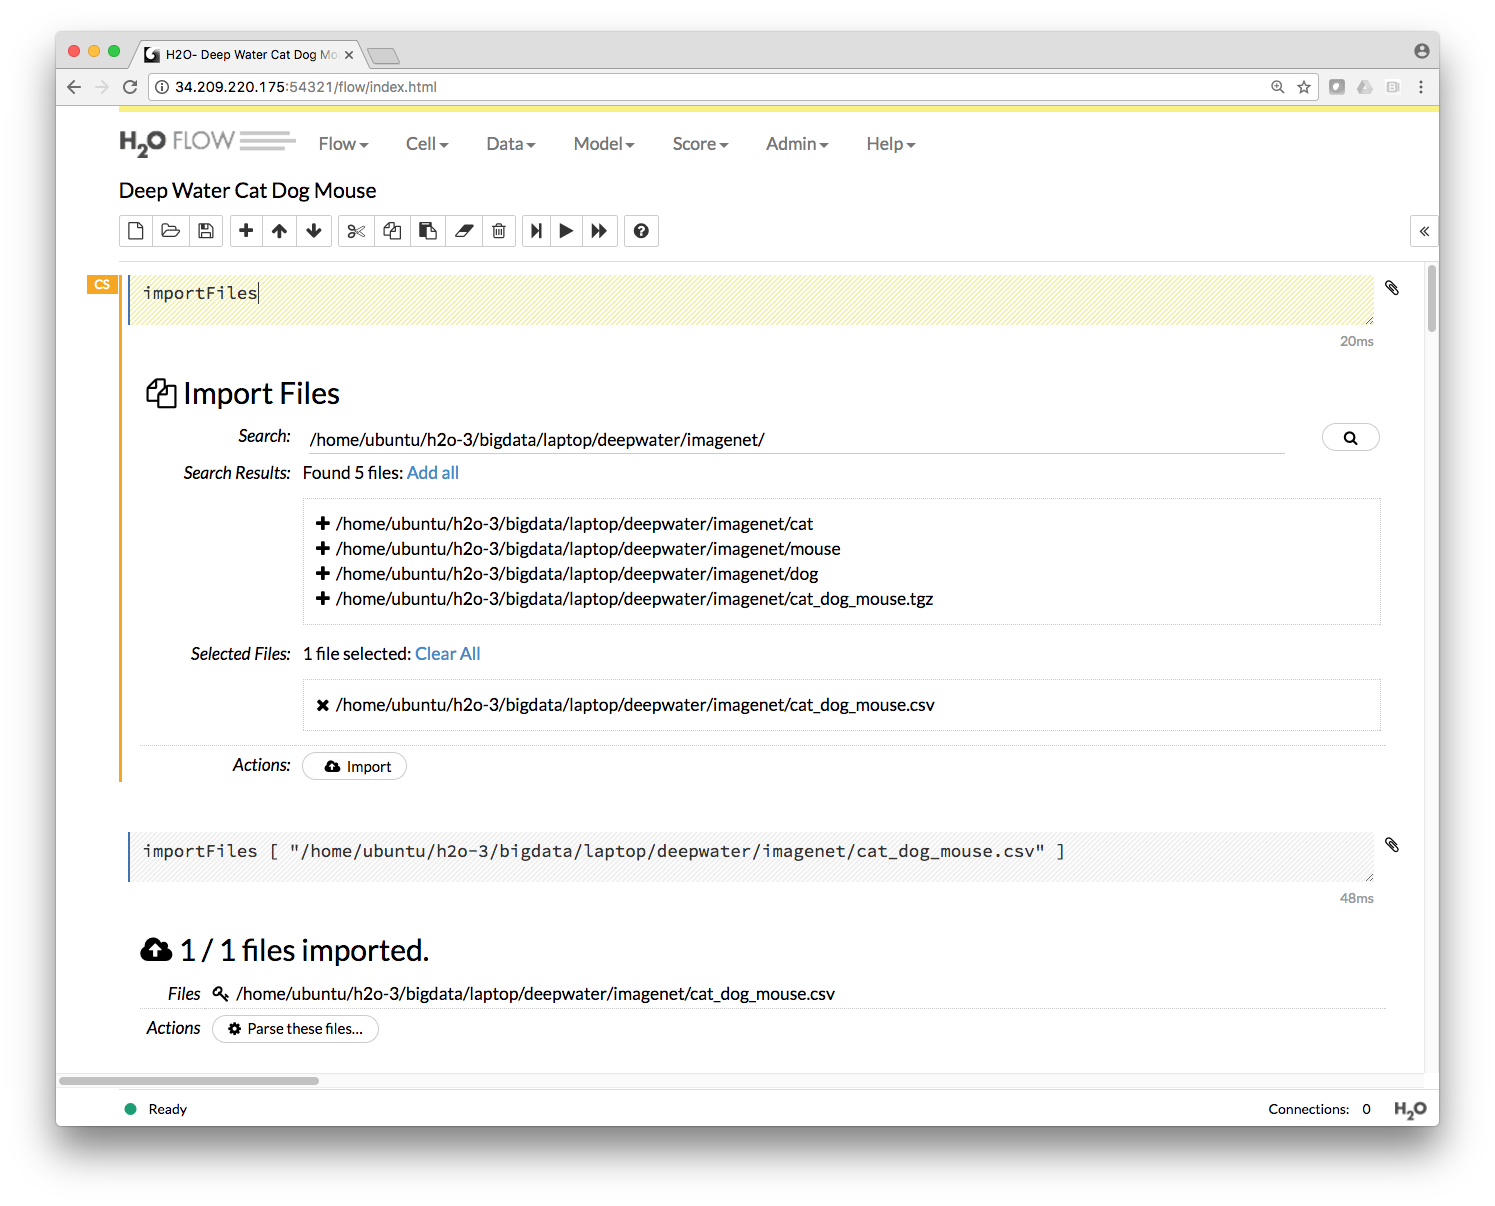
\includegraphics[width=0.77\textwidth]{images/flow-import-data.png}
		\caption{Import data}\label{fig:flow-import-data}
	\end{center}
	\end{figure}
	
	\newpage
	\begin{figure}[H]
	\begin{center}
		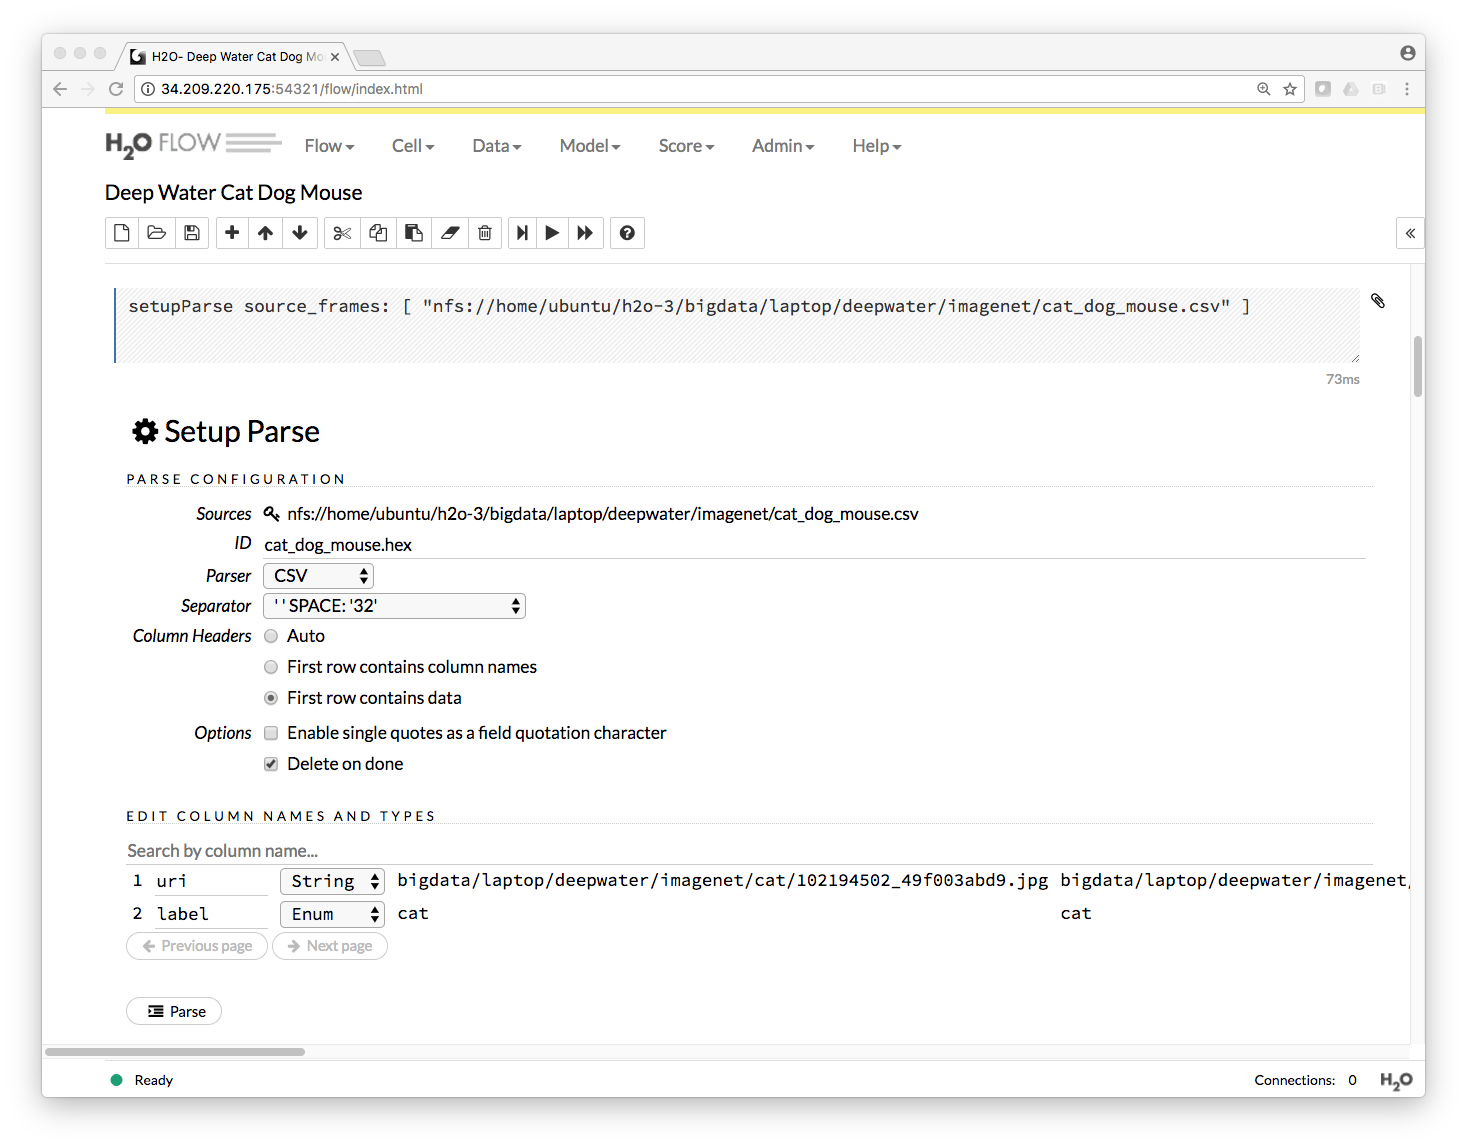
\includegraphics[width=0.77\textwidth]{images/flow-parse-data.png}
		\caption{Parse data}\label{fig:flow-parse-data}
	\end{center}
	\end{figure}
	
	\begin{figure}[H]
	\begin{center}
		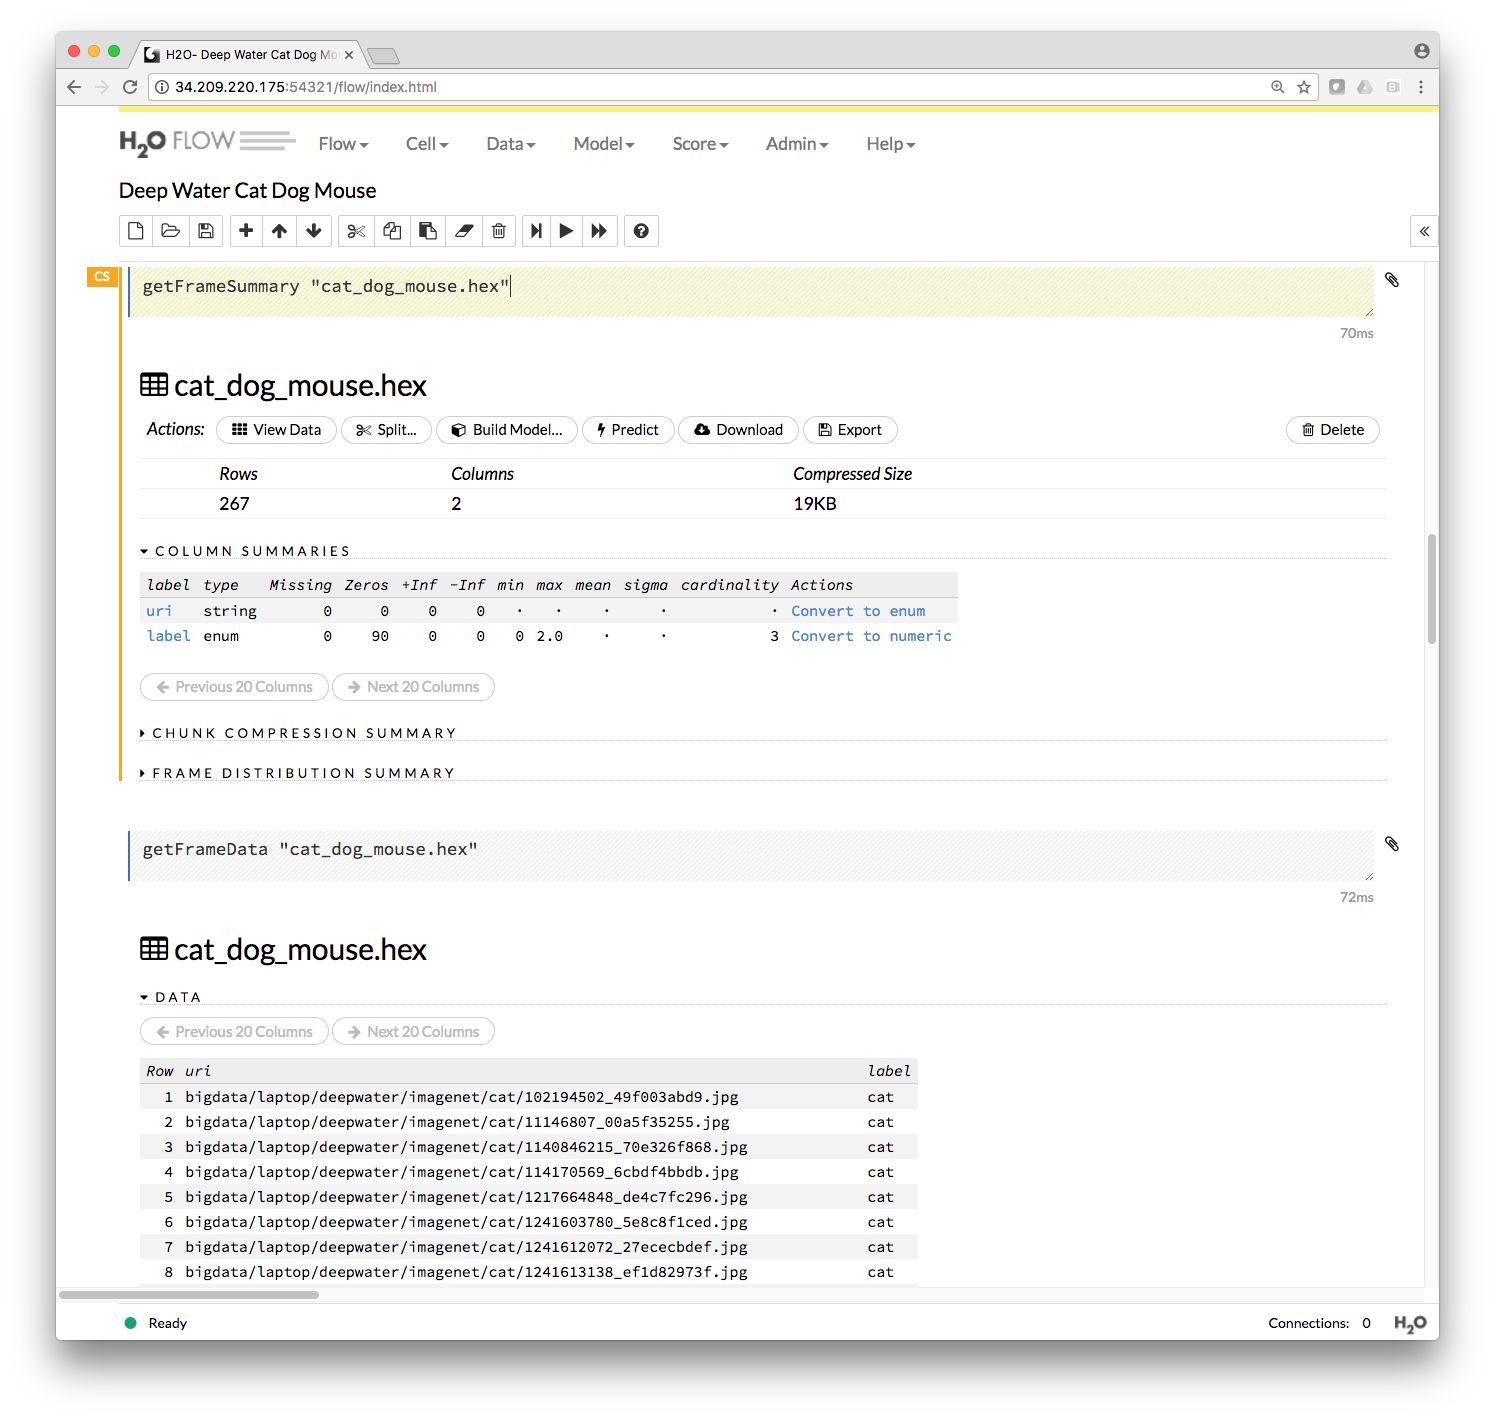
\includegraphics[width=0.77\textwidth]{images/flow-view-data.png}
		\caption{View data}\label{fig:flow-view-data}
	\end{center}
	\end{figure}
	
	\newpage
	A Deep Water model is built just like any other H2O algorithm as shown in Figure \ref{fig:flow-build-dw-model}.  In this example, we use a simple LeNet  pre-defined network. (Refer to \textit{\citetalias{lenet}} \cite{lenet}.) Best practice defaults are set for all parameters.  Figures \ref{fig:flow-backend} and \ref{fig:flow-gpu} highlight the key backend and GPU selection parameters in the Deep Water Flow configuration, respectively.
	
	\begin{figure}[H]
	\begin{center}
		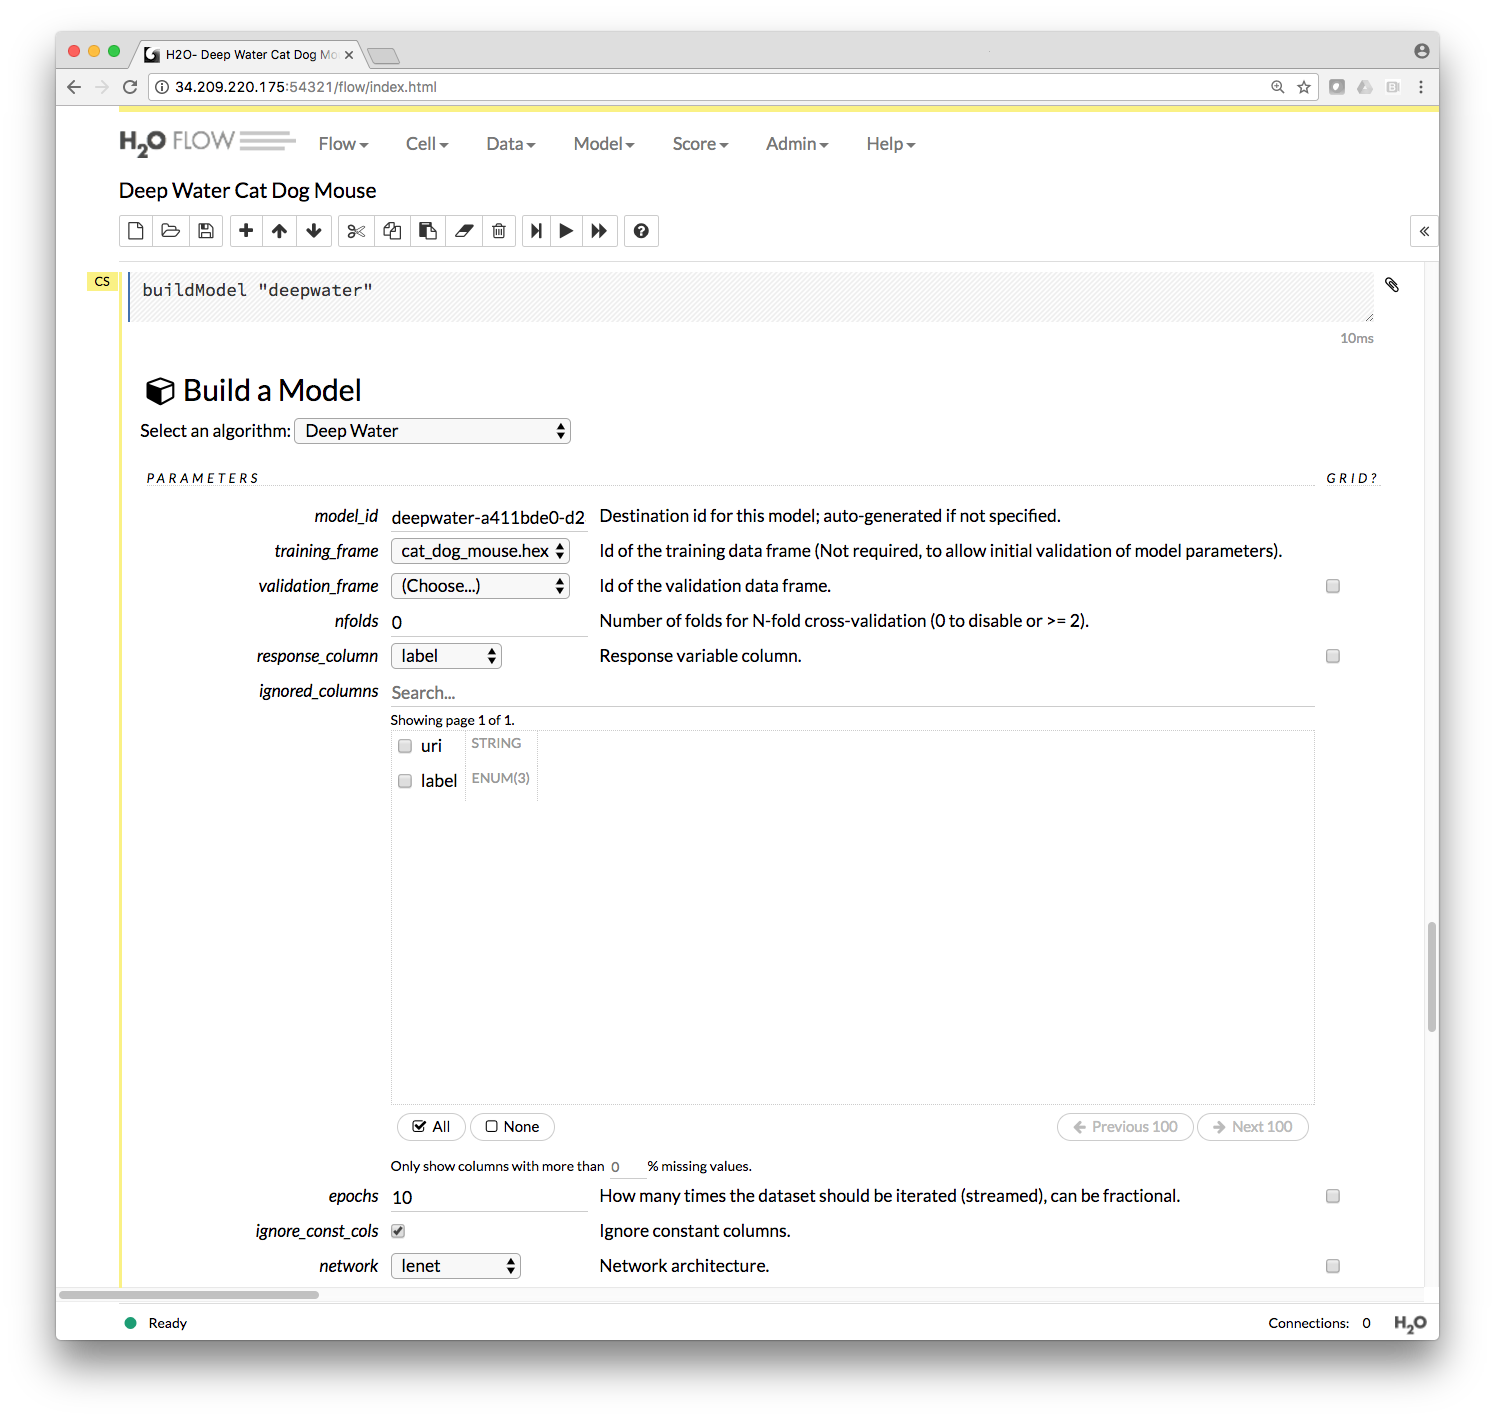
\includegraphics[width=0.77\textwidth]{images/flow-build-dw-model.png}
		\caption{Build Deep Water model}\label{fig:flow-build-dw-model}
	\end{center}
	\end{figure}
	
	\newpage
	\begin{figure}[H]
	\begin{center}
		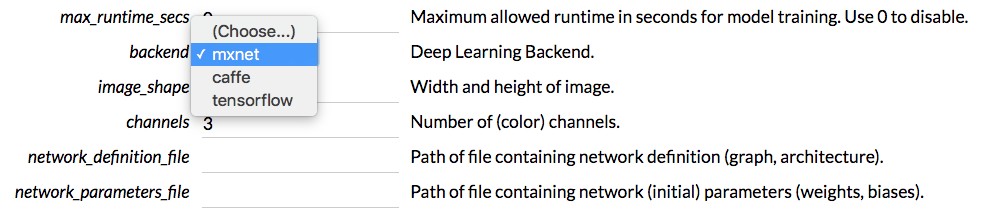
\includegraphics[width=\textwidth]{images/flow-backend.png}
		\caption{Deep Water backend options}\label{fig:flow-backend}
	\end{center}
	\end{figure}
	\begin{figure}[H]
	\begin{center}
		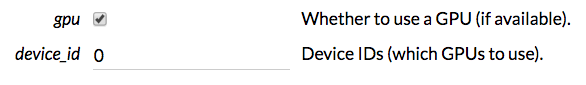
\includegraphics[width=0.7\textwidth]{images/flow-gpu.png}
		\caption{Deep Water GPU selection}\label{fig:flow-gpu}
	\end{center}
	\end{figure}

\newpage
\section{Grid Search}
	H2O's grid search API can be used with Deep Water.  Grid search allows users to specify sets of values for parameter arguments and observe changes in model behavior.  This is useful for hyperparameter tuning.  For all grid searches, the type of search and early stopping can be configured to stop searches if there is no substantial metric improvement in searches after successive rounds.  Search criteria (\texttt{search\_criteria}) are passed as a dictionary to the grid search class:
	\begin{itemize}
		\item{\texttt{strategy}}: Specify \texttt{"Cartesian"} (default), \texttt{"RandomDiscrete"}
		\item{\texttt{stopping\_metric}}: Specify the metric to use for early stopping.
		\item{\texttt{stopping\_rounds}}: Specify early stopping based on convergence of the \texttt{stopping\_metric}.  Stop if the simple moving average of length $k$ of the \texttt{stopping\_metric} does not improve from $k$ \texttt{stopping\_rounds} scoring events. (Use 0 to disable.)
		\item{\texttt{stopping\_tolerance}}: Specify relative tolerance for metric-based stopping criterion. (Stop if relative improvement is not at least this much.)
	\end{itemize}
	
	You can read more about grid search in the \textbf{\href{https://blog.h2o.ai/2016/06/hyperparameter-optimization-in-h2o-grid-search-random-search-and-the-future/}{Hyperparameter Optimization in H2O}} blog at \texttt{https://blog.h2o.ai/2016/06/hyperparameter-} \texttt{optimization-in-h2o-grid-search-random-search-and-the-} \\ \texttt{future/}.
	
	\newpage
	\subsection{Cartesian Search}
		A cartesian grid search will run a model for each combination of parameters in the grid.  In the example below, two sets of hidden layers and two learning rates are specified in the grid, which will result in four models being built.
		
\waterExampleInPython
\lstinputlisting[style=python, linerange=7-27]{DW_Vignette_code_examples/mnist-grid-cart.py}

	\newpage
	\subsection{Random Search}
		The hyperparameter search space can become too large to compute exhaustively. Given a fixed amount of time, making random choices of hyperparameter values can give results that are on par with or even better than the best results of a Cartesian search. (See \textit{\citetalias{bergstra-bengio}} \cite{bergstra-bengio}.) This example expands the search space for hidden layers and learning rate and adds a parameter for input dropout. The max search time is set to five minutes.
		
\waterExampleInPython
\lstinputlisting[style=python, linerange=15-30]{DW_Vignette_code_examples/mnist-grid-random.py}

\section{Model Checkpoints}
Model checkpoints are useful in saving models (i.e. training state) for long training runs or to resume model training, sometimes with different parameters.  In the example below, a model is trained for 20 epochs and then saved via the \texttt{h2o.save\_model} method.  The model is then restored via the \texttt{h2o.load\_model} method, and training is resumed.

\waterExampleInPython
\lstinputlisting[style=python, linerange=7-39]{DW_Vignette_code_examples/mnist-chkpt.py}

\newpage
\section{Ensemble}
Deep Water models can be ensembled with other models built with H2O, leveraging the rich algorithmic capabilities of the H2O machine learning platform.  Below, three base learners are built with 5-fold cross-validation: GBM, GLM, and Deep Water. The base learners are then ensembled together via the stacking method. You can read more about stacking here: {\url{http://docs.h2o.ai/h2o/latest-stable/h2o-docs/data-science/stacked-ensembles.html}}.

\waterExampleInPython
\lstinputlisting[style=python]{DW_Vignette_code_examples/mnist-ensemble.py}

\newpage
\section{Deep Features and Similarity}
The hidden layers of a trained model can provide a useful feature representation of input data.  A Deep Water model's \texttt{deepfeatures} method allows you to extract hidden layer feature representations of input data.  These extracted feature representations can be used in several ways.  In the example below, features are extracted from a layer of a pre-trained convolutional network. (Refer to \textit{\citetalias{inceptionbn}} \cite{inceptionbn}.)  The extracted features are then used to train a multinomial GLM model.

\waterExampleInPython
\lstinputlisting[style=python, linerange=12-32]{DW_Vignette_code_examples/cdm-deepfeatures.py}

\lstinputlisting[style=python, linerange=20-29]{DW_Vignette_code_examples/cdm-deepfeatures.txt}

Another use of hidden layer feature representation is for unsupervised applications, such as clustering or recommendations.  The deep features are used as vector representations whereby similarity measures can be computed.  Given two H2OFrames \texttt{X} and \texttt{Y}, the following will compute a resultant H2OFrame whereby a similarity measure, specified by the \texttt{similarity} parameter, is computed for each vector in \texttt{X} and \texttt{Y}: \texttt{X.distance(Y, similarity)}.\\
\\
We can express this mathematically.

\begin{equation*}
\begin{aligned}
	\mathbf{X} &=
		\begin{bmatrix}
			x_{1,1}	&	\dots	&	x_{1,P}\\
			\vdots	&	\ddots	&	\vdots\\
			x_{N,1}	&	\dots	&	x_{N,P}
		\end{bmatrix}, \text{ where } \mathbf{x}_i = [x_{i,1}, \dots, x_{i,P}]\\
	\mathbf{Y} &= \begin{bmatrix}
		y_{1,1}	&	\dots	&	y_{1,P}\\
		\vdots	&	\ddots	&	\vdots\\
		y_{M,1}	&	\dots	&	y_{M,P}
	\end{bmatrix}, \text{ where } \mathbf{y}_i = [y_{i,1}, \dots, y_{i,P}]\\
\end{aligned}
\end{equation*}


$\mathbf{distance}\left(\mathbf{X}, \mathbf{Y}\right) = \mathbf{Z} : z_{i,j} = \mathbf{similarity}\left(\mathbf{x}_i,\mathbf{y}_j\right)$, where $\mathbf{X} \in \mathbb{R}^{N \times P}, \mathbf{Y} \in \mathbb{R}^{M \times P}, \mathbf{Z} \in \mathbb{R}^{N \times M}$

\newpage
The following are the various similarity measures that can be computed.

$\ell_1$ similarity (\texttt{"l1"}): $z_{i,j} = \displaystyle\sum_{k=1}^P|x_{i,k} - y_{j,k}|$\\
$\ell_2$ similarity (\texttt{"l2"}): $z_{i,j} = \sqrt{\displaystyle\sum_{k=1}^P(x_{i,k} - y_{j,k})^2}$\\
cosine similarity (\texttt{"cosine"}): $z_{i,j} = \displaystyle\frac{\mathbf{x}_i \cdot \mathbf{y}_j}{||\mathbf{x}_i||_2||\mathbf{y}_j||_2} = \frac{\displaystyle\sum_{k=1}^P x_{i,k} y_{j,k}}{\sqrt{\displaystyle\sum_{k=1}^Px_{i,k}^2}\sqrt{\displaystyle\sum_{k=1}^Py_{j,k}^2}}$\\
cosine squared similarity (\texttt{"cosine\_sq"}): $z_{i,j} = \left(\displaystyle\frac{\mathbf{x}_i \cdot \mathbf{y}_j}{||\mathbf{x}_i||_2||\mathbf{y}_j||_2}\right)^2$
\\
\\
The following code snippet uses the same extracted features from the previous example.  This time, the extracted features frame is split into two frames, the first three rows/vectors become a \texttt{queries} frame, and the rest of the rows/vectors are assigned to a \texttt{references} frame.  A similarity frame is created between the \texttt{references} and \texttt{queries} frames, where each element $x_{i,j}$ is the similarity measure between \texttt{reference} vector $i$ and \texttt{queries} vector $j$.

\waterExampleInPython
\lstinputlisting[style=python, linerange=19-32]{DW_Vignette_code_examples/cdm-similarity.py}

\newpage
The following is the output of the code snippet.

\lstinputlisting[style=python, linerange=20-36]{DW_Vignette_code_examples/cdm-similarity.txt}

\section{Multi-GPU}
Multi-GPU support is available through backend-specific mechanisms.  For example, in TensorFlow, multi-GPU specification can be done through the computational graph.  For examples, please visit: {\url{https://github.com/h2oai/h2o-3/tree/master/examples/deeplearning/notebooks}}.

\section{Deployment for Inference}
	\subsection{Model Object Optimized (MOJO)}
		With H2O, you can convert your deep water models into a binary model object optimized (MOJO) formats. This format is easily embeddable in any Java environment and independent of an H2O cluster.  The only compilation and runtime dependencies for generated models are the \texttt{h2o-genmodel.jar} and the \texttt{deepwater-all.jar} files, which are produced as part of the build output.  Deep Water models can be exported as a MOJO and embedded in a custom Java application.  You can read more about MOJOs here: {\url{http://docs.h2o.ai/h2o/latest-stable/h2o-genmodel/javadoc/index.html}}.\\
		\\
		Deep Water MOJOs can be downloaded from H2O Flow by clicking \textbf{Download Model Deployment Package} from a Deep Water model. (See Figure \ref{fig:flow-mojo}.)  From the Python API, you can use the \texttt{download\_mojo} method for a model.  For example: 
		
		\begin{verbatim}
		model.download_mojo(path="/path/to/model_mojo", 
		                    get_genmodel_jar=True)
		\end{verbatim}
		
		\begin{figure}[H]
		\begin{center}
			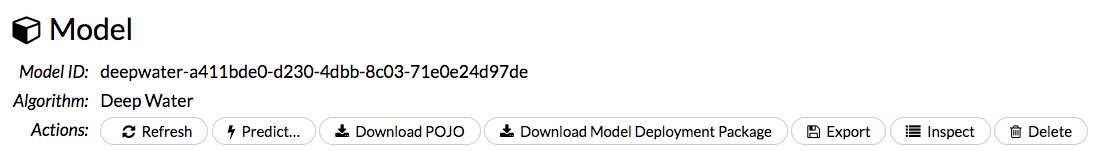
\includegraphics[width=\textwidth]{images/flow-mojo.png}
			\caption{Deep Water model actions}\label{fig:flow-mojo}
		\end{center}
		\end{figure}

	\subsection{Prediction Service Builder}
		The H2O Prediction Service Builder is a standalone web service application that can help users compile MOJOs and build Web Archive (War) files for prediction web services.  The details of how to build the H2O Prediction Service Builder can be found here:  {\url{https://github.com/h2oai/steam/tree/master/prediction-service-builder}}.
		
		Before generating a War file, be sure that you have both the \texttt{h2o-genmodel.jar} and \texttt{deepwater-all.jar} files. You can obtain each of these by running the following:
		
\texttt{\small{curl localhost:54321/3/h2o-genmodel.jar > h2o-genmodel.jar}}\\
\texttt{\small{curl localhost:54321/3/deepwater-all.jar > deepwater-all.jar}}


		War files can be generated using the Prediction Service Builder Web UI or via command line.  For example, submitting the following command submits the necessary dependencies to the Prediction Server Builder (running on localhost on port 55000) to create an \texttt{example.war} file.

\begin{verbatim}
curl -X POST \
--form mojo=@mojo.zip \
--form jar=@h2o-genmodel.jar \
--form deepwater=@deepwater-all.jar \
localhost:55000/makewar > example.war
\end{verbatim}

		The \texttt{example.war} file can be started using an appropriate Jetty runner.  For example, the following command starts the prediction service on port 55001: 
    		\small{\texttt{java -jar jetty-runner-9.3.9.M1.jar --port 55001 example.war}} 
		
		Upon completion, a prediction service for scoring will be available at \\
		{\texttt{http://localhost:55001}}.


\section{Upcoming}
At the time of this writing, we have many exciting upcoming releases and initiatives at H2O.ai.
	\begin{itemize}
		\item{\textbf{Machine Learning and GPUs}}: H2O.ai has developed the fastest scalable, distributed in-memory machine learning platform, and we now extend its capabilities to GPUs, aiming to create the fastest artificial intelligence platform on GPUs.  Stay tuned for more of our algorithms exploiting GPU-acceleration.
		\item{\textbf{Automatic Machine Learning}}: H2O AutoML is an automatic machine learning capability that will encapsulate and automate best practices in data cleaning, feature engineering, hyper-parameter search, and ensemble generation.
		\item{\textbf{Machine Learning Interpretability}}: Often times, especially in regulated industries, model transparency and explanation become just as paramount as predictive performance.  Through visualizations and various techniques, machine learning interpretability functionality will continually make its way to the H2O platform.  For details on the ideas around machine learning interpretability, please visit: {\url{https://www.oreilly.com/ideas/ideas-on-interpreting-machine-learning}}.
	\end{itemize}

\section{Acknowledgements}

We would like to acknowledge the following individuals for their contributions to and review of this booklet: Jo-Fai (Joe) Chow, Megan Kurka, Erin LeDell, Ray Peck, Patrick Hall, and Surekha Jadhwani. 

\section{Errata}
This version of H2O Deep Water is still a pre-release version. An errata document is available, describing current known issues that you might encounter when trying out Deep Water. This document is available in the h2o-3 GitHub repo at {\url{https://github.com/h2oai/h2o-3/blob/master/h2o-docs/src/booklets/source/DeepWaterBookletErrata.md}}. 

If the Errata document does not answer your question, feel free to post your question to Stack Overflow using the \textbf{h2o} tag at {\url{http://stackoverflow.com/questions/tagged/h2o}}.


\section{References}
\bibliographystyle{plainnat}

\nobibliography{bibliography.bib} %hides entire bibliography so just \bibentry items are included - use \bibentry{bibname} (where bibname is the entry name in the bibliography) to include entries from bibliography.bib; double brackets {{ are required in .bib file to preserve capitalization


\begin{enumerate}

	\item{\bibentry{h2o_DL_booklet}}

	\item{\bibentry{bergstra-bengio}}

	\item{\bibentry{resnet}}

	\item{\bibentry{inceptionbn}}

	\item{\bibentry{alexnet}}

	\item{\bibentry{mnist}}

	\item{\bibentry{lenet}}

	\item{\bibentry{vgg}}

	\item{\bibentry{googlenet}}
		
\end{enumerate}

\newpage
\section{Authors}

\textbf{Wen Phan}

Wen Phan is a senior solutions architect at H2O.ai. Wen works with customers and organizations to architect systems, smarter applications, and data products to make better decisions, achieve positive outcomes, and transform the way they do business. Wen holds a B.S. in electrical engineering and M.S. in analytics and decision sciences.  Follow him on Twitter: @wenphan

\textbf{Magnus Stensmo}

Magnus has been a scientist and software engineer in workplaces ranging from new startups to large companies. Using machine learning and information retrieval, he has built numerous systems for internet and enterprise software companies, including large scale real-time similarity search, product recommendation systems, text analysis, and medical and machine diagnosis.  Magnus holds a PhD in Computer Science and an MSc in Computer Science and Engineering from the Royal Institute of Technology (KTH) in Stockholm, Sweden. He has also studied neuroscience, philosophy, business, and linguistics.

\textbf{Mateusz Dymczyk}

Mateusz is a software developer who loves all things distributed, machine learning, and data juggling.  He obtained his M.Sc. in Computer Science from AGH UST in Krakow, Poland, during which he did an exchange at L’ECE Paris in France and worked on distributed flight booking systems. After graduation, he moved to Tokyo, where he is still currently based, to work as a researcher at Fujitsu Laboratories on machine learning and NLP projects. In his spare time, he tries to be part of the IT community by organizing, attending, and speaking at conferences and meet ups.  Follow him on Twitter: @mdymczyk.

\textbf{Arno Candel}

Arno is the Chief Technology Officer of H2Oa.ai. He is also the main author of H2O Deep Learning.  Arno holds a PhD and a Masters summa cum laude in Physics from ETH Zurich, Switzerland. He has authored dozens of scientific papers and is a sought-after conference speaker. Arno was named ��2014 Big Data All-Star by Fortune Magazine. Follow him on Twitter: @ArnoCandel.

\textbf{Qiang Kou}

Qiang Kou was an early developer for Deep Water.  He is currently pursuing his PhD in informatics at Indiana University.  Qiang is also an Rcpp core team member and Apache MXNet committer.  Follow him on Twitter: @KKusingR

\end{document}
